\chapter{绪论}
\section{研究背景及意义}
\subsection{课题研究背景}
\subsubsection{SDN}
SDN
TE
TE 与 SDN的结合


\subsubsection{NFV}


在传统的网络架构中,数据平面和控制平面没有分离,是集成在同一处的硬件系统上的。这使得新业务在引进时十分不便,一方面需要在路由交换、数据处理等业务之外进行相关处理工作,宁一方面还需要在网络技术、支撑软件与业务创建软件等软件相关方面进行相应地设计与研究。这样来,使得网络运营商需要增加成本来进行运营维护,也阻碍了客户要求的队业务作出迅速响应的请求,同时也妨碍了业务的创新。

传统网络的层次结构是互联网取得巨大成功的关键.但是随着网络规模的不断扩大,封闭的网络设备内置了过多的复杂协议,增加了运营商定制优化网络的难度,科研人员无法在真实环境中规模部署新协议.同时,互联网流量的快速增长(预计到2018 年,全球流量将达到1.6*1021 字节[1]),用户对流量的需求不断扩大,各种新型服务不断出现,增加了网络运维成本.换机下发统一标准规则,交换机仅需按照这些规则执行相应的动作即可.因此,SDN 技术能够有效降低设备负载,协助网络运营商更好地控制基础设施,降低整体运营成本,成为最具前途的网络技术之一.因此,SDN 被MIT列为“改变世界的十大创新技术之一”[5].SDN 相关技术研究迅速开展起来,成为近年来的研究热点.2013 年,SIGCOMM 会议收录了多篇相关文章,甚至将SDN 列为专题来研讨,带动了SDN 相关研究的蓬勃发展.

随着网络的快速发展,传统互联网出现了如传统网络配置复杂度高等诸多问题[6],这些问题说明网络架构需要革新,可编程网络的相关研究为SDN 的产生提供了可参考的理论依据[7].主动网络[8,9]允许数据包携带用户程序,并能够由网络设备自动执行.用户可以通过编程方式动态地配置网络,达到了方便管理网络的目的.然而由于需求低、协议兼容性差等问题,并未在工业界实际部署.4D 架构[10,11]将可编程的决策平面(即控制层)从数据平面分离,使控制平面逻辑中心化与自动化,其设计思想产生SDN 控制器的雏形[12].
借鉴计算机系统的抽象结构,未来的网络结构将存在转发抽象、分布状态抽象和配置抽象这3 类虚拟化概念[13].转发抽象剥离了传统交换机的控制功能,将控制功能交由控制层来完成,并在数据层和控制层之间提供了标准接口,确保交换机完成识别转发数据的任务.控制层需要将设备的分布状态抽象成全网视图,以便众多应用能够通过全网信息进行网络的统一配置.配置抽象进一步简化了网络模型,用户仅需通过控制层提供的应用接口对网络进行简单配置,就可自动完成沿路径转发设备的统一部署.因此,网络抽象思想解耦了路径依赖,成为数据控制分离且接口统一架构(即SDN)产生的决定因素.此外,众多标准化组织已经加入到SDN相关标准的制订当中.专门负责订制SDN接口标准的著名组织是开
放网络基金会(Open Networking Foundation,简称ONF)[14],该组织制订的OpenFlow 协议业已成为SDN 接口的主流标准,许多运营商和生产厂商根据该标准进行研发.互联网工程任务组(Internet Engineering Task Force,简称IETF) 的ForCES 工作组[15]、互联网研究专门工作组(Internet Research Task Force,简称IRTF)的SDNRG 研究组[16]以及国际电信联盟远程通信标准化组织(ITU Telecommunication Standardization Sector,简称ITU-T)的多个工作组[17]同样针对SDN 的新方法和新应用等展开研究.标准化组织的跟进,促使了SDN 市场的快速发展.据悉,SDN 市场已于2013 年达到约2 亿美元的产值,预计到2016 年将达到20 亿美元[18],市场需求确保SDN 有足够的发展空间.由此可见,SDN 具有广阔的发展前景和巨大的研究价值.

QoS 约束的链路故障多备份路径恢复算法


随着通信技术的快速发展,网络链路带宽得到不断扩充。目前全球至少有来自20 多个国家的53个运营商已经部署或正在考虑部署 400 GB/s 的骨
干网络[1]。高速骨干网链路即使短暂的故障也会造成
大量的数据包丢弃,严重影响通信质量。根据对ISP
的观察,骨干网链路一年内大约有30%的概率会出
现故障[2],表明链路故障是网络中较为普遍的现象。
因此,加快故障的恢复速度,降低故障造成的业务
丢弃已成为当前研究亟待解决的问题。
网络故障主要表现为链路故障,链路故障恢复
策略可分为主动式和被动式两种[3,4]。被动式策略在
网络故障后动态自适应地进行全网资源重分配,但
路由重新收敛花费较多的时间而不可接受。因此目
前故障快速恢复研究以主动式策略为主,通过提前
对网络进行资源规划和预留,使得故障时能迅速切
换,如基于多拓扑[5]和基于备份路径的故障恢复技
术。多拓扑技术需要配置多个拓扑子层,路由存储
消耗大;基于备份路径的故障恢复技术提供端到端
路径重路由,在全局范围内进行流量分配,易于基
于现有协议实现。因此,备份路径技术是当前故障
恢复领域研究的热点[6-11]。
故障恢复的本质在于维持故障链路承载流量的
传输,因此应从流量持续传输角度解决故障恢复问
题。大部分故障恢复工作集中在如何选择可靠备份
路径上,且一般利用单一备份路径进行故障恢复。
然而当流量超出备份路径可用带宽时,单一备份路
径无法满足故障恢复的要求。受到这一启发,文献
[8]将多路径技术引入到故障恢复中,采用多条备份
路径共同承担流量,减少了流量的丢弃。在此基础
上,文献[9]提出一种结合故障恢复与流量工程的网
络结构,在多路径故障恢复基础上进行流量工程优
化,其目的是进行负载均衡,且假设备份路径可用
带宽满足故障恢复需求。文献[10]考虑了不同故障状
况,通过将重路由流量分配给有跳数限制的多条备
份路径,在网络投入运行之前就设计好应对各种故
障场景的最低容量备份网络。文献[11]提出一种跨层
故障恢复模型,考虑了备份链路的可靠性,提升了
故障恢复成功率。然而,上述故障恢复算法大都以
最大化重路由为目标,未考虑恢复后的流量是否满
足用户的需求。但是经由备份路径的重路由流量即
使最终传输成功,由于时延超时、链路过载等原因,
也无法满足业务的服务质量需求(Quality of Service,
QoS),属于无效流量。虽然文献[12]提出了一种满
足QoS 约束的自适应调整的多路径路由,但未考虑
故障恢复问题。因此,目前已提出的大部分链路故
障恢复算法不能很好地确保业务的服务质量。
为此,本文针对QoS 约束下的链路故障恢复问
题进行研究,即在网络可用带宽和业务时延需求约
束下进行最大化重路由流量问题求解。首先基于多
备份路径策略建立概率关联故障模型和重路由流量
丢弃优化目标,并构建QoS 约束的故障多备份路径
恢复问题的数学优化模型。然后,设计QoS 约束的
链路故障多备份路径恢复算法(Multiple backup
Paths Recovery for link failure with QoS constrain
algorithm, MPR-QoS) 对此问题进行求解。
MPR-QoS 算法在构建单条备份路径时,利用改进
的QoS 约束的k 最短路径法进行拼接,并以最大化
减少重路由流量丢弃为目标,且分配给高优先级链
路更多的保护资源。此外还证明了算法的正确性并
对时间空间复杂度进行了分析。最后,在NS2 仿真
环境下从故障恢复率、重路由流量QoS 满足率、链
路过载率和算法运行时间等方面验证了本文算法的
优越性。


SDN作为新型网络架构,数据网络中心作为未来网络研究的重要领域,SDN在数据中心网络的应用具有研究意义。

本文结合实际情况,以基于SDN网络的多路径路由技术作为课题的研究方向,主要研究以三个方面内容。


\subsection{课题研究目的和意义}


\section{预备知识}
\subsection{图论}
网络通常表示为图$G(\mathbb{V},\mathbb{E})$,其中$\mathbb{V}$是$|\mathbb{V}|$个节点的集合(例如,节点表示路由)和$\mathbb{E}$是$|\mathbb{E}|$条链路的集合(例如,链路代表光纤线路或无线电信道)。链接可能带有延迟、长度或成本等属性。对于每条链路$e_i$,$w_{e_i}$表示链路的权重。路径$P$的权重表示为路径$P$中每条链路的权重之和$w_P=\sum\limits_{e_i\in \mathbb{P}}w_{e_i}$。

共享风险链接组(SRLG)是一组链路共享同一个组件,该组件的故障会导致所有链路的故障。一条链接可以属于多个共享风险链接组里。举个例子,在光网络的导管中\cite{bhandari1994optimal}可以放置多条光链路,如图.\ref{fig:Logic shift operation}所示,链路(1,2),(3,2)和(3,4)放置在一个导管中,同时链路(3,2)和(3,4)也共同放置在另一个导管中。如果某个导管被切断,相应导管的链路将失效。每个导管对应一个共享风险链接组。其它共享风险链接组的应用是交通网络的相关拥塞和电网的级联故障\cite{coudert2007shared}。


\begin{figure}[htbp]
\centering
\subfigure[Physical topology with conduit]{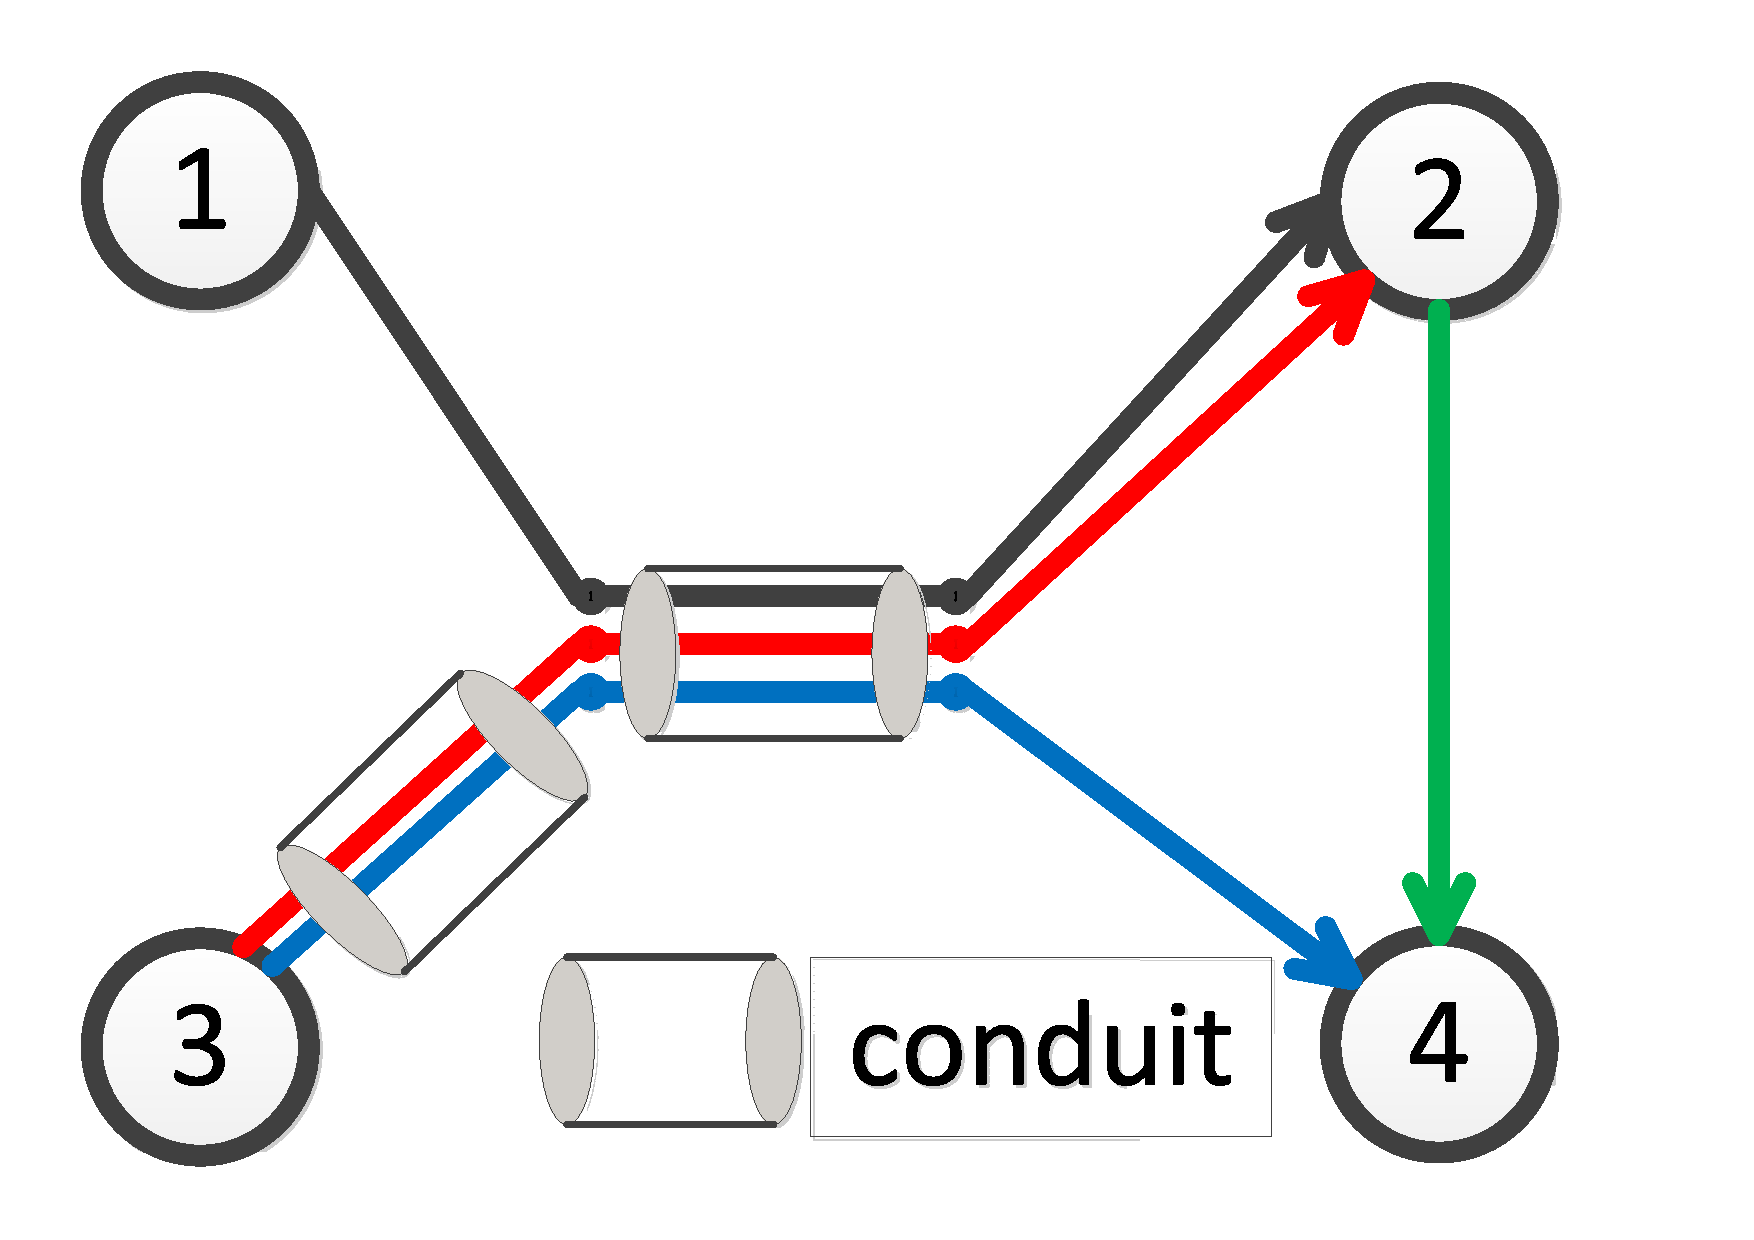
\includegraphics[width=1.25 in]{figures/PhysicalGraph}
}
\subfigure[Network Graph]{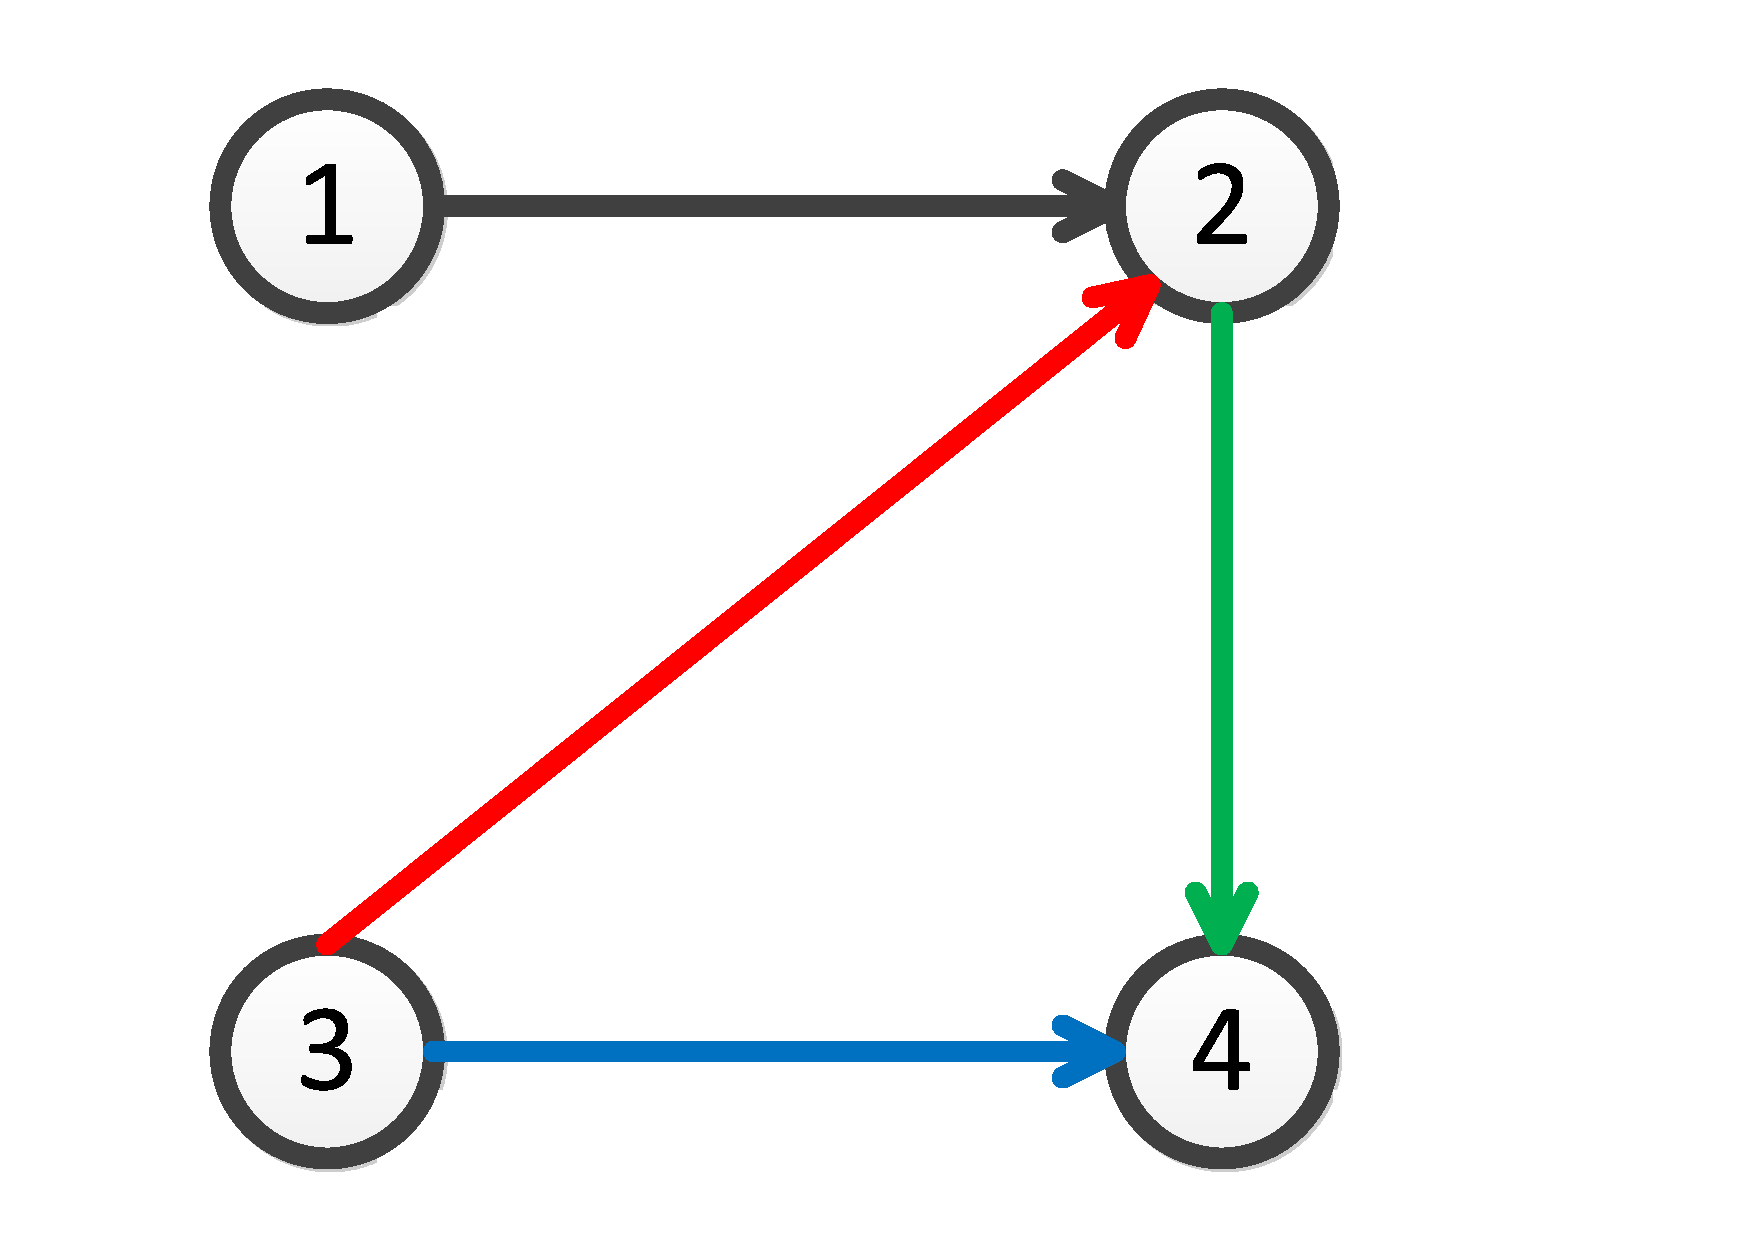
\includegraphics[width=0.9 in]{figures/VirtualGraph}
}
\caption{Example of shared risk link group(SRLG)}\label{fig:SRLGgraph}
\label{fig:Logic shift operation}
\end{figure}

设$\mathbb{R}$为网络中的风险集(故障)。每个风险可能对应于导管断开、光纤断裂、在一个节点上驱动故障、软件故障或这些因素的任何组合。对每一个共享风险链路组$r_i \in \mathbb{R}$是指与其风险$r_i$相关的链路集合$\mathbb{R}_{r_i}$,$1\leq i\leq \chi$ 和 $\chi=|{\mathbb{R}}|$是共享风险链路组集合的个数。图.\ref{fig:CompositeGraph}(a)所示,该图包含五个共享风险链路组集合$\mathbb{R}_{r_1}=\{e_1,e_9\}$, $\mathbb{R}_{r_2}=\{e_2,e_3,e_{19}\}$, $\mathbb{R}_{r_3}=\{e_2,e_4,e_{11},e_{17}\}$, $\mathbb{R}_{r_4}=\{e_5,e_{13}\}$, $\mathbb{R}_{r_5}=\{e_{15},e_{18}\}$。在这个例子中,链路$e_2$同属两个共享风险链路组集合里$\mathbb{R}_{r_2}$ 和 $\mathbb{R}_{r_3}$


$r_P$表示影响路径$P$上的风险集合,即$r_P=\{r\in \mathbb{R}$: 路径 $P$ 包含的链路在 $\mathbb{R}_r$中$\}$。如图.\ref{fig:CompositeGraph}(c)所示,在路径$AP$ 上的边集$\mathbb{AP}=\{e_1,e_2,e_3,e_4,e_5,e_6,e_7,e_8\}$,并且$e_1\in \mathbb{R}_{r_1}$, $e_2\in \mathbb{R}_{r_2}$, $e_2\in \mathbb{R}_{r_3}$, $e_3\in \mathbb{R}_{r_2}$, $e_4\in \mathbb{R}_{r_3}$, $e_5\in \mathbb{R}_{r_4}$,路径$AP$的风险集合是${r}_{{AP}}=\{r_1, r_2, r_3, r_4\}$。$\mathbb{\mathbb{ER}}$代表不属于$AP$上的链路但是与$AP$共享相同的风险集合的链路。如图.\ref{fig:CompositeGraph}(c)所示,$\mathbb{\mathbb{ER}}=\{e_9,e_{11},e_{17},e_{13},e_{19}\}$。




\subsubsection{最大网络流}
\label{subsubsec:maxFlow}
设$G=(\mathbb{\mathbb{V}},\mathbb{\mathbb{E}})$是一个网络(其中$\mathbb{\mathbb{V}}$是$|\mathbb{\mathbb{V}}|$个节点的集合,$\mathbb{\mathbb{E}}$是$|\mathbb{\mathbb{E}}|$条链路的集合),其中$s\in \mathbb{V}$和$d\in \mathbb{V}$分别指源节点和终节点。链路$e_i$ 的\textbf{容量}表示该条链路的最大流量。链路的流$f_{e_i}$应该满足以下两个限制:
\begin{enumerate}
  \item 容量限制: $\forall e_i\in \mathbb{\mathbb{E}}$: $f_{e_i}\leq c_{e_i}$.
  \item 流量守恒: $\forall u\in \mathbb{\mathbb{V}}-\{s,d\}$: $\sum\limits_{v\in \mathbb{V}}f_{(v,u)}=\sum\limits_{v\in \mathbb{V}}f_{(u,v)}$,  $(v,u)$ 和 $(u,v)$ 代表链路 $e(v,u)$ 和 $e(u,v)$.
\end{enumerate}

流的值定义为$|f|=\sum\limits_{v\in \mathbb{V}}f_{(s,v)}$,其中s是源节点。它表示从s节点到d节点的流量。\textbf{最大流量问题}:尽可能的求从s节点到d节点的最大流量值$|f|$。

一个 s-d 割${\Phi}=(\mathbb{S},\mathbb{D})$ 是节点$\mathbb{V}$的划分满足$s \in \mathbb{S}$ 和 $d \in \mathbb{D}$。$\Phi$ 的割集合$\mathbb{\mathbb{L}}_{\Phi}$是一个包含边的集合。
\begin{equation}
\mathbb{\mathbb{L}}_{\Phi}=\{(u,v)\in \mathbb{E}: u \in \mathbb{S}, v \in \mathbb{D}\}.
\end{equation}

如果在割集合$\mathbb{\mathbb{L}}_{\Phi}$中的边被去除,那么在原图中的流值$|f| = 0$。即没有流能从s节点到d节点。一个 s-d 割${\Phi}=(\mathbb{S},\mathbb{D})$的容量被定义成$c(\Phi)=\sum\limits_{e_i\in \mathbb{\mathbb{L}}_{\Phi}}c_{e_i}$。\textbf{最小s-d 割 $\Phi$ 问题},最小化$c(\Phi)$即决定点集$\mathbb{S}$ 和 $\mathbb{D}$使得s-d割${\Phi}=(\mathbb{S},\mathbb{D})$的($c(\Phi)$) 最小化 。

\textbf{最小割最大流定理}:一个s-d流的最大值等于s-d割的最小割。如图.\ref{fig:FlowNetwork}所示,在图$G$中的流量$|f|=f_{(s,v_1)}+f_{(s,v_2)}$。这个割$\Phi(\mathbb{S},\mathbb{D})$ 是 $\mathbb{S}=\{s,v_1,v_2,v_4\}$ 和$\mathbb{D}=\{v_3,d\}$,它是最小的割其容量为$c(\Phi)=c_{(v_1,v_3)}+c_{(v_4,v_3)}+c_{(v_4,d)}=12+7+4=23$. 显然, $|f|=c(\Phi)$, 即s-d 最大流等于所有s-d割中最小的容量。
\begin{figure}[htbp]
  \centering
  % Requires \usepackage{graphicx}
  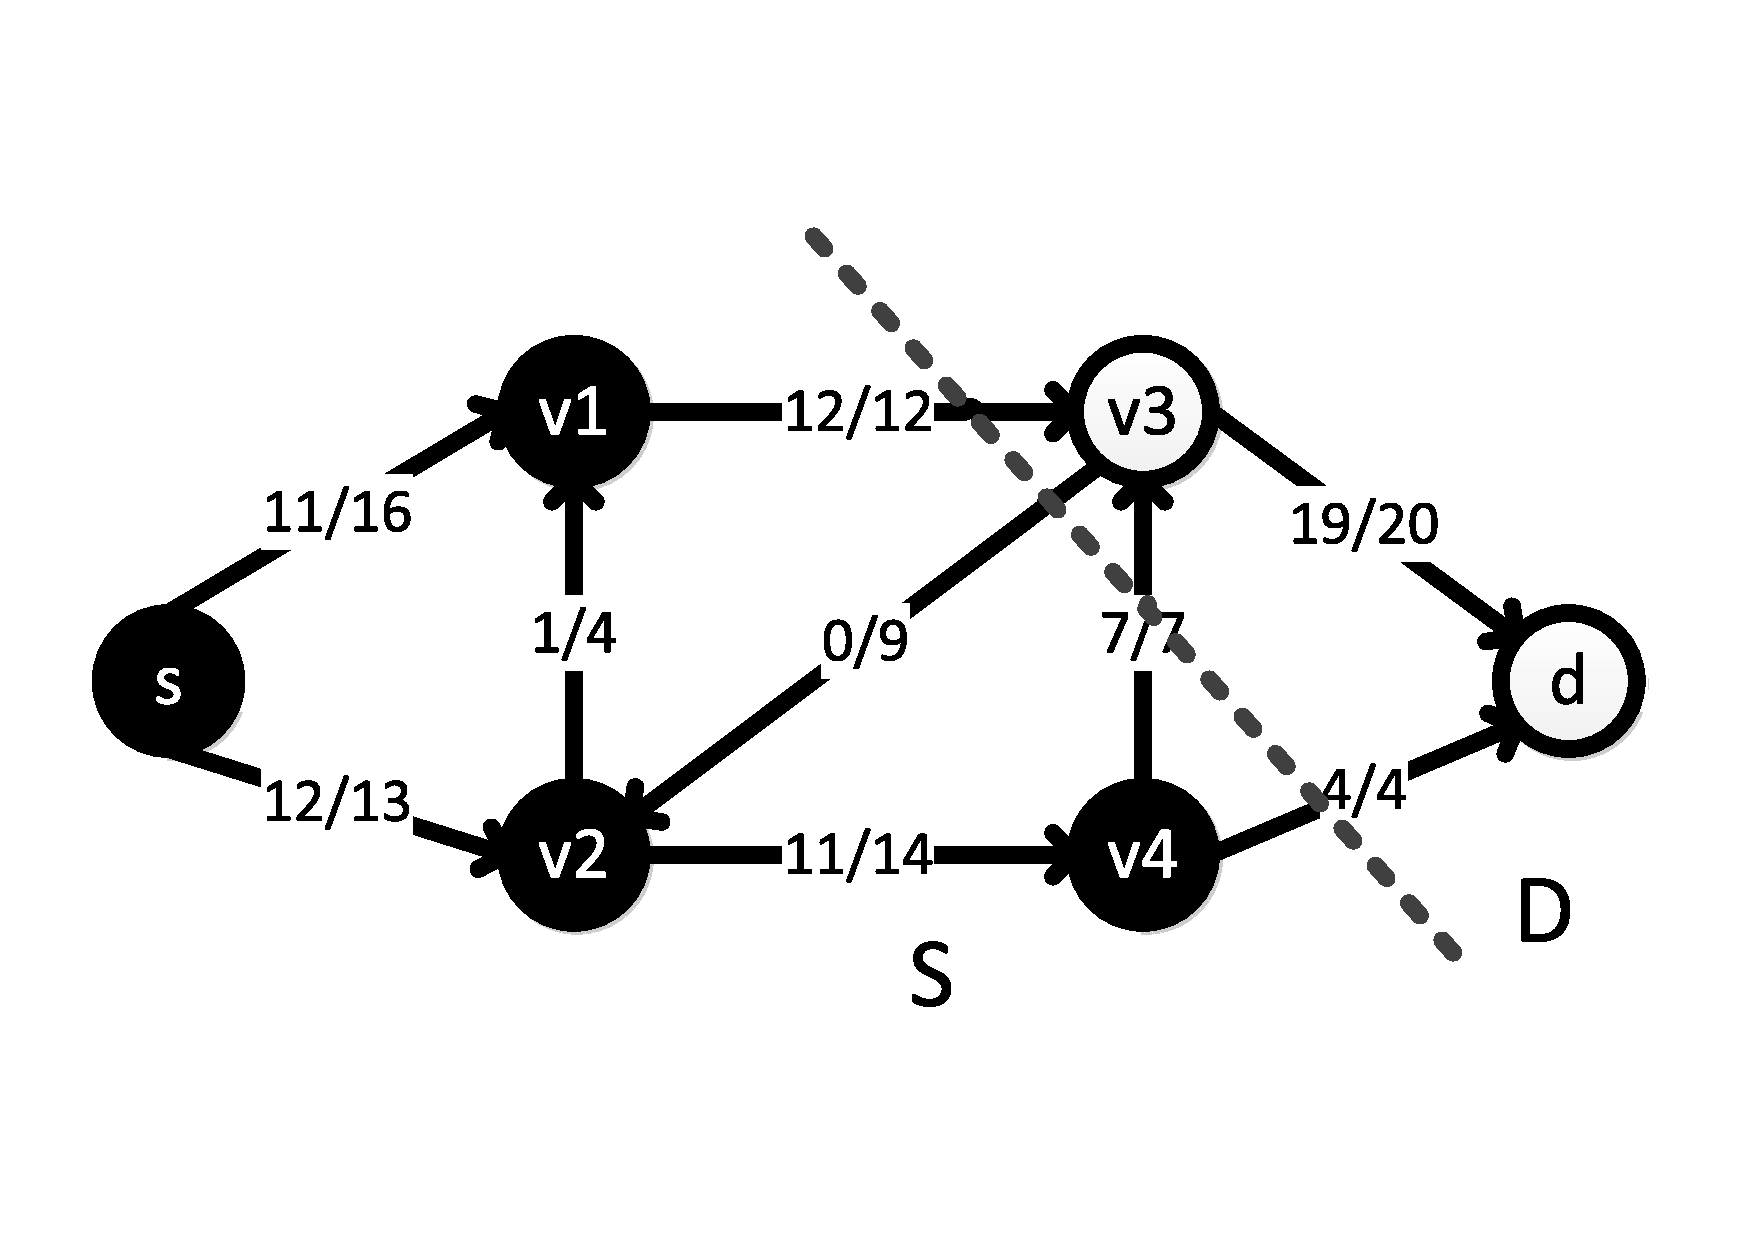
\includegraphics[width=2.5in]{figures/FlowNetwork}\\
  \caption{An example to illustrate max-flow min-cut theorem. Each link $e_i$ is labeled by $f_{e_i}/c_{e_i}$, where $f_{e_i}$ and $c_{e_i}$ denote the flow and capacity of link $e_i$, respectively.   }
  \label{fig:FlowNetwork}
\end{figure}

\subsection{计算理论}

\section{相关的研究及发展趋势}


\section{论文的主要研究内容和组织结构}
\subsection{论文的主要研究内容}
\subsection{论文的组织结构与贡献}
本文依据SDN、路由算法以及分离路径。。等方面的研究现状与发展趋势,并结合自身对以上的研究和探索,将本文分为五章,各章主要内容如下:
\begin{itemize}
  \item 第一章为绪论部分,主要介绍了本课题的研究背景及其意义并且简要地分析了国内外研究现状和发展趋势。
  \item 介绍
  \item 介绍
\end{itemize}


